% Source: StudentGovernmentRepo/Common_Sense_Carolina_Lobbying_org/figures/funding_model.tex
\documentclass[border=15pt]{standalone}
\usepackage{tikz}
\usepackage{pgfplots}
\usepackage{xcolor}
\usetikzlibrary{positioning, arrows.meta, calc, fit, backgrounds, decorations.markings}
\pgfplotsset{compat=1.18}
\definecolor{garnet}{HTML}{73000A}
\definecolor{sandstorm}{HTML}{FFF2E3}
\definecolor{rose}{HTML}{CC2E40}
\definecolor{atlantic}{HTML}{466A9F}
\definecolor{congaree}{HTML}{1F414D}
\definecolor{horseshoe}{HTML}{65780B}
\definecolor{honeycomb}{HTML}{A49137}
\definecolor{warmgrey}{HTML}{676156}
\definecolor{tenblack}{HTML}{ECECEC}

\begin{document}
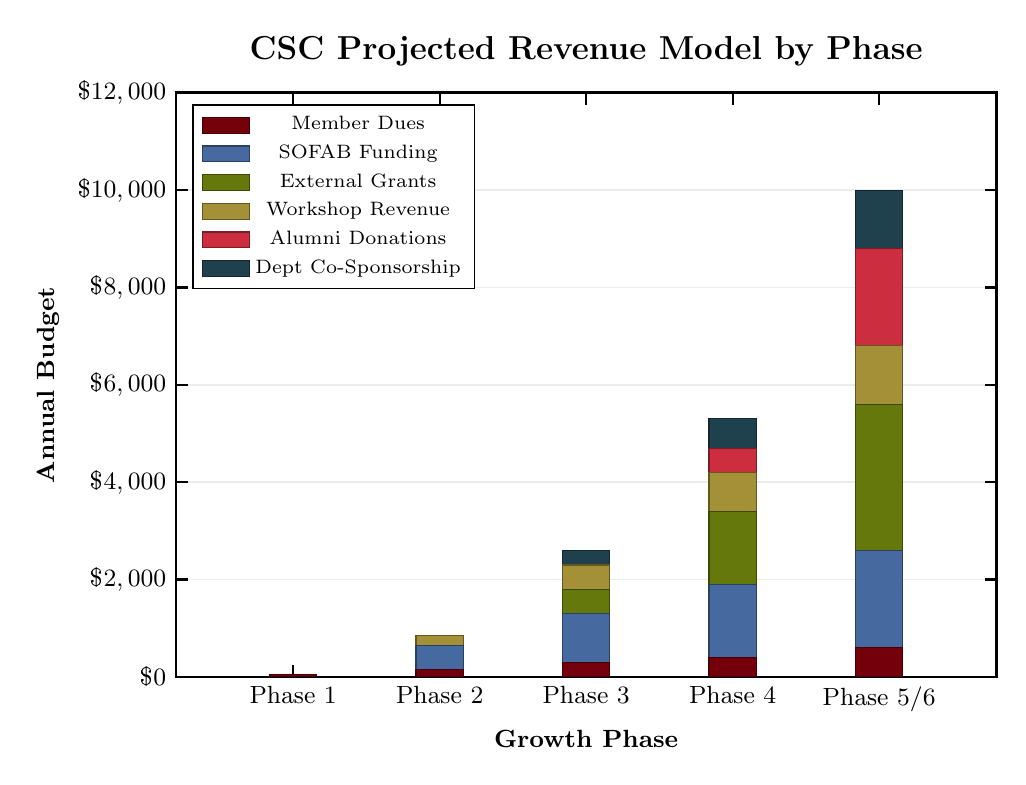
\begin{tikzpicture}

\begin{axis}[
  title={CSC Projected Revenue Model by Phase},
  title style={font=\bfseries\large},
  width=12cm,
  height=9cm,
  ybar stacked,
  bar width=0.6cm,
  ylabel={Annual Budget},
  xlabel={Growth Phase},
  ylabel style={font=\small\bfseries},
  xlabel style={font=\small\bfseries},
  symbolic x coords={Phase 1, Phase 2, Phase 3, Phase 4, Phase 5/6},
  xtick=data,
  xticklabel style={font=\small},
  ymin=0,
  ymax=12000,
  ytick={0,2000,4000,6000,8000,10000,12000},
  scaled y ticks=false,
  yticklabel={\$\pgfmathprintnumber[fixed, precision=0, 1000 sep={,}]{\tick}},
  yticklabel style={font=\small},
  enlarge x limits=0.2,
  ymajorgrids=true,
  grid style={tenblack, line width=0.6pt},
  axis line style={line width=1pt, black},
  tick style={line width=0.8pt, black},
  legend style={
    at={(0.02,0.98)},
    anchor=north west,
    font=\scriptsize,
    draw=black,
    fill=white,
    rounded corners=0pt,
    line width=0.6pt,
    /tikz/every even column/.append style={column sep=0.15cm}
  },
  area legend,
]

% 1. Member Dues (garnet)
\addplot[fill=garnet, draw=garnet!60!black, line width=0.4pt] coordinates {
  (Phase 1,  50)
  (Phase 2, 150)
  (Phase 3, 300)
  (Phase 4, 400)
  (Phase 5/6, 600)
};
\addlegendentry{Member Dues}

% 2. SOFAB Funding (atlantic)
\addplot[fill=atlantic, draw=atlantic!60!black, line width=0.4pt] coordinates {
  (Phase 1,    0)
  (Phase 2,  500)
  (Phase 3, 1000)
  (Phase 4, 1500)
  (Phase 5/6, 2000)
};
\addlegendentry{SOFAB Funding}

% 3. External Grants (horseshoe)
\addplot[fill=horseshoe, draw=horseshoe!60!black, line width=0.4pt] coordinates {
  (Phase 1,    0)
  (Phase 2,    0)
  (Phase 3,  500)
  (Phase 4, 1500)
  (Phase 5/6, 3000)
};
\addlegendentry{External Grants}

% 4. Workshop Revenue (honeycomb)
\addplot[fill=honeycomb, draw=honeycomb!60!black, line width=0.4pt] coordinates {
  (Phase 1,   0)
  (Phase 2, 200)
  (Phase 3, 500)
  (Phase 4, 800)
  (Phase 5/6, 1200)
};
\addlegendentry{Workshop Revenue}

% 5. Alumni Donations (rose)
\addplot[fill=rose, draw=rose!60!black, line width=0.4pt] coordinates {
  (Phase 1,    0)
  (Phase 2,    0)
  (Phase 3,    0)
  (Phase 4,  500)
  (Phase 5/6, 2000)
};
\addlegendentry{Alumni Donations}

% 6. Dept Co-Sponsorship (congaree)
\addplot[fill=congaree, draw=congaree!60!black, line width=0.4pt] coordinates {
  (Phase 1,   0)
  (Phase 2,   0)
  (Phase 3, 300)
  (Phase 4, 600)
  (Phase 5/6, 1200)
};
\addlegendentry{Dept Co-Sponsorship}

\end{axis}

\end{tikzpicture}
\end{document}
